\documentclass{standalone}
\usepackage{tikz}
\usetikzlibrary{patterns, positioning}


\begin{document}
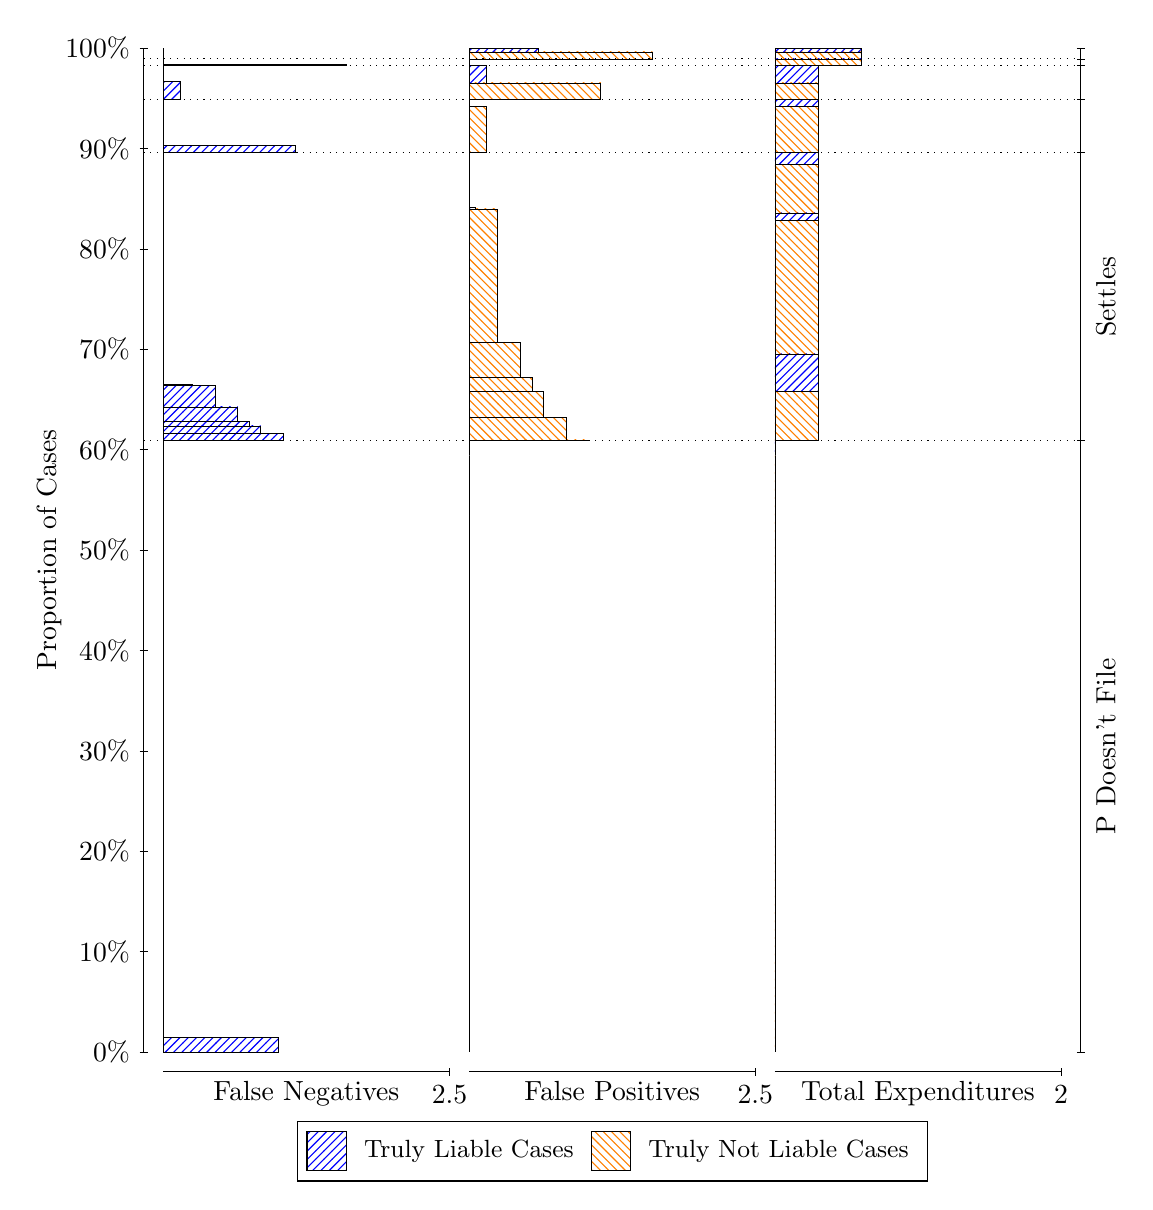
\begin{tikzpicture}
\draw[black, very thin] (1.5,1.75) -- (1.5,14.5);
\node[rotate=90, text=black, anchor=center] at (0.3, 8.125) {Proportion of Cases};
\draw[black, very thin] (1.45,1.75) -- (1.55,1.75);
\node[text=black, anchor=east] at (1.45, 1.75) {0\%};
\draw[black, very thin] (1.45,3.025) -- (1.55,3.025);
\node[text=black, anchor=east] at (1.45, 3.025) {10\%};
\draw[black, very thin] (1.45,4.3) -- (1.55,4.3);
\node[text=black, anchor=east] at (1.45, 4.3) {20\%};
\draw[black, very thin] (1.45,5.575) -- (1.55,5.575);
\node[text=black, anchor=east] at (1.45, 5.575) {30\%};
\draw[black, very thin] (1.45,6.85) -- (1.55,6.85);
\node[text=black, anchor=east] at (1.45, 6.85) {40\%};
\draw[black, very thin] (1.45,8.125) -- (1.55,8.125);
\node[text=black, anchor=east] at (1.45, 8.125) {50\%};
\draw[black, very thin] (1.45,9.4) -- (1.55,9.4);
\node[text=black, anchor=east] at (1.45, 9.4) {60\%};
\draw[black, very thin] (1.45,10.675) -- (1.55,10.675);
\node[text=black, anchor=east] at (1.45, 10.675) {70\%};
\draw[black, very thin] (1.45,11.95) -- (1.55,11.95);
\node[text=black, anchor=east] at (1.45, 11.95) {80\%};
\draw[black, very thin] (1.45,13.225) -- (1.55,13.225);
\node[text=black, anchor=east] at (1.45, 13.225) {90\%};
\draw[black, very thin] (1.45,14.5) -- (1.55,14.5);
\node[text=black, anchor=east] at (1.45, 14.5) {100\%};

\draw[black, very thin] (13.4,1.75) -- (13.4,14.5);
\draw[black, very thin] (13.35,1.75) -- (13.45,1.75);
\node[anchor=west] at (13.35, 1.75) {};
\draw[black, very thin] (13.35,9.5143) -- (13.45,9.5143);
\node[anchor=west] at (13.35, 9.5143) {};
\draw[black, very thin] (13.35,13.172) -- (13.45,13.172);
\node[anchor=west] at (13.35, 13.172) {};
\draw[black, very thin] (13.35,13.846) -- (13.45,13.846);
\node[anchor=west] at (13.35, 13.846) {};
\draw[black, very thin] (13.35,14.283) -- (13.45,14.283);
\node[anchor=west] at (13.35, 14.283) {};
\draw[black, very thin] (13.35,14.362) -- (13.45,14.362);
\node[anchor=west] at (13.35, 14.362) {};
\draw[black, very thin] (13.35,14.5) -- (13.45,14.5);
\node[anchor=west] at (13.35, 14.5) {};

\draw[black, very thin, pattern color=blue, pattern=north east lines] (1.75,1.75) rectangle (3.2033,1.9368);
\draw[black, very thin, pattern color=orange, pattern=north west lines] (1.75,1.9368) rectangle (1.75,9.5143);
\draw[black, very thin, pattern color=blue, pattern=north east lines] (1.75,9.5143) rectangle (3.276,9.6077);
\draw[black, very thin, pattern color=blue, pattern=north east lines] (1.75,9.6077) rectangle (2.9853,9.7007);
\draw[black, very thin, pattern color=blue, pattern=north east lines] (1.75,9.7007) rectangle (2.84,9.757);
\draw[black, very thin, pattern color=blue, pattern=north east lines] (1.75,9.757) rectangle (2.6947,9.9439);
\draw[black, very thin, pattern color=blue, pattern=north east lines] (1.75,9.9439) rectangle (2.404,10.214);
\draw[black, very thin, pattern color=blue, pattern=north east lines] (1.75,10.214) rectangle (2.1133,10.23);
\draw[black, very thin, pattern color=orange, pattern=north west lines] (1.75,10.23) rectangle (1.75,13.172);
\draw[black, very thin, pattern color=blue, pattern=north east lines] (1.75,13.172) rectangle (3.4213,13.262);
\draw[black, very thin, pattern color=orange, pattern=north west lines] (1.75,13.262) rectangle (1.75,13.846);
\draw[black, very thin, pattern color=blue, pattern=north east lines] (1.75,13.846) rectangle (1.968,14.072);
\draw[black, very thin, pattern color=orange, pattern=north west lines] (1.75,14.072) rectangle (1.75,14.283);
\draw[black, very thin, pattern color=blue, pattern=north east lines] (1.75,14.283) rectangle (4.0753,14.293);
\draw[black, very thin, pattern color=orange, pattern=north west lines] (1.75,14.293) rectangle (1.75,14.362);
\draw[black, very thin, pattern color=orange, pattern=north west lines] (1.75,14.362) rectangle (1.75,14.452);
\draw[black, very thin, pattern color=blue, pattern=north east lines] (1.75,14.452) rectangle (1.75,14.5);
\draw[black, very thin, pattern color=orange, pattern=north west lines] (5.6333,1.75) rectangle (5.6333,9.3275);
\draw[black, very thin, pattern color=blue, pattern=north east lines] (5.6333,9.3275) rectangle (5.6333,9.5143);
\draw[black, very thin, pattern color=orange, pattern=north west lines] (5.6333,9.5143) rectangle (7.1593,9.5247);
\draw[black, very thin, pattern color=orange, pattern=north west lines] (5.6333,9.5247) rectangle (6.8687,9.8133);
\draw[black, very thin, pattern color=orange, pattern=north west lines] (5.6333,9.8133) rectangle (6.578,10.142);
\draw[black, very thin, pattern color=orange, pattern=north west lines] (5.6333,10.142) rectangle (6.4327,10.319);
\draw[black, very thin, pattern color=orange, pattern=north west lines] (5.6333,10.319) rectangle (6.2873,10.76);
\draw[black, very thin, pattern color=orange, pattern=north west lines] (5.6333,10.76) rectangle (5.9967,12.457);
\draw[black, very thin, pattern color=blue, pattern=north east lines] (5.6333,12.457) rectangle (5.706,12.473);
\draw[black, very thin, pattern color=blue, pattern=north east lines] (5.6333,12.473) rectangle (5.6333,13.172);
\draw[black, very thin, pattern color=orange, pattern=north west lines] (5.6333,13.172) rectangle (5.8513,13.757);
\draw[black, very thin, pattern color=blue, pattern=north east lines] (5.6333,13.757) rectangle (5.6333,13.846);
\draw[black, very thin, pattern color=orange, pattern=north west lines] (5.6333,13.846) rectangle (7.3047,14.058);
\draw[black, very thin, pattern color=blue, pattern=north east lines] (5.6333,14.058) rectangle (5.8513,14.283);
\draw[black, very thin, pattern color=orange, pattern=north west lines] (5.6333,14.283) rectangle (5.6333,14.353);
\draw[black, very thin, pattern color=blue, pattern=north east lines] (5.6333,14.353) rectangle (5.6333,14.362);
\draw[black, very thin, pattern color=orange, pattern=north west lines] (5.6333,14.362) rectangle (7.9587,14.452);
\draw[black, very thin, pattern color=blue, pattern=north east lines] (5.6333,14.452) rectangle (6.5053,14.5);
\draw[black, very thin, pattern color=orange, pattern=north west lines] (9.5167,1.75) rectangle (9.5167,9.3275);
\draw[black, very thin, pattern color=blue, pattern=north east lines] (9.5167,9.3275) rectangle (9.5167,9.5143);
\draw[black, very thin, pattern color=orange, pattern=north west lines] (9.5167,9.5143) rectangle (10.062,10.142);
\draw[black, very thin, pattern color=blue, pattern=north east lines] (9.5167,10.142) rectangle (10.062,10.615);
\draw[black, very thin, pattern color=orange, pattern=north west lines] (9.5167,10.615) rectangle (10.062,12.311);
\draw[black, very thin, pattern color=blue, pattern=north east lines] (9.5167,12.311) rectangle (10.062,12.405);
\draw[black, very thin, pattern color=orange, pattern=north west lines] (9.5167,12.405) rectangle (10.062,13.023);
\draw[black, very thin, pattern color=blue, pattern=north east lines] (9.5167,13.023) rectangle (10.062,13.172);
\draw[black, very thin, pattern color=orange, pattern=north west lines] (9.5167,13.172) rectangle (10.062,13.757);
\draw[black, very thin, pattern color=blue, pattern=north east lines] (9.5167,13.757) rectangle (10.062,13.846);
\draw[black, very thin, pattern color=orange, pattern=north west lines] (9.5167,13.846) rectangle (10.062,14.058);
\draw[black, very thin, pattern color=blue, pattern=north east lines] (9.5167,14.058) rectangle (10.062,14.283);
\draw[black, very thin, pattern color=orange, pattern=north west lines] (9.5167,14.283) rectangle (10.607,14.353);
\draw[black, very thin, pattern color=blue, pattern=north east lines] (9.5167,14.353) rectangle (10.607,14.362);
\draw[black, very thin, pattern color=orange, pattern=north west lines] (9.5167,14.362) rectangle (10.607,14.452);
\draw[black, very thin, pattern color=blue, pattern=north east lines] (9.5167,14.452) rectangle (10.607,14.5);
\draw[black, dotted] (1.5,9.5143) -- (13.4,9.5143);
\draw[black, dotted] (1.5,13.172) -- (13.4,13.172);
\draw[black, dotted] (1.5,13.846) -- (13.4,13.846);
\draw[black, dotted] (1.5,14.283) -- (13.4,14.283);
\draw[black, dotted] (1.5,14.362) -- (13.4,14.362);
\draw[black, very thin] (1.75,1.5) -- (5.3833,1.5);
\node[text=black, anchor=north] at (3.5667, 1.5) {False Negatives};
\draw[black, very thin] (5.3833,1.45) -- (5.3833,1.55);
\node[text=black, anchor=north] at (5.3833, 1.45) {2.5};

\draw[black, very thin] (5.6333,1.5) -- (9.2667,1.5);
\node[text=black, anchor=north] at (7.45, 1.5) {False Positives};
\draw[black, very thin] (9.2667,1.45) -- (9.2667,1.55);
\node[text=black, anchor=north] at (9.2667, 1.45) {2.5};

\draw[black, very thin] (9.5167,1.5) -- (13.15,1.5);
\node[text=black, anchor=north] at (11.333, 1.5) {Total Expenditures};
\draw[black, very thin] (13.15,1.45) -- (13.15,1.55);
\node[text=black, anchor=north] at (13.15, 1.45) {2};

\node[text=black, centered, rotate=90] at (13.72, 5.6321) {P Doesn't File};
\node[text=black, centered, rotate=90] at (13.72, 11.343) {Settles};





\draw (7.449999999999999,1.5) node[draw=none] (baseCoordinate) {};
\begin{scope}[align=center]
        \matrix[scale=0.5, draw=black, below=0.5cm of baseCoordinate, nodes={draw}, column sep=0.1cm]{
            \node[rectangle, draw, minimum width=0.5cm, minimum height=0.5cm, pattern color=blue, pattern=north east lines] {}; &
            \node[draw=none, font=\small, text=black] (B) {Truly Liable Cases}; &
            \node[rectangle, draw, minimum width=0.5cm, minimum height=0.5cm, pattern color=orange, pattern=north west lines] {}; &
            \node[draw=none, font=\small, text=black] (B) {Truly Not Liable Cases}; \\
            };
\end{scope}

\end{tikzpicture}
\end{document}